% ===========================================================================
% Section 2 -- Instances and generator
% ===========================================================================

We test on two sources of instances: ten instances adapted from a public
benchmark (Section~\ref{sec:orlib}) and a family of instances from our own
scalable generator (Sections~\ref{sec:generator}--\ref{sec:suite}). All
instances are stored in a common JSON format (duty start/end times, the arc
list of $G$, $W$ and $T$), and the models read only these fields.

\subsection{Existing benchmarks}
\label{sec:orlib}

We found no public benchmark for exactly this problem: half-time and
full-time employees with a fixed cost per employee and two separate limits on
working time and total time. Two related families exist.

\paragraph{Bus driver scheduling (BDSP).} Kletzander and
Musliu~\cite{kletzander2020} introduced a benchmark based on an Austrian
collective agreement. Its rules (break placement, driving blocks, cost
depending on the hours paid) are much richer than ours, and the original
real-world data cannot be published. We could only use it by discarding most
of its structure, so we did not adopt it.

\paragraph{OR-Library crew scheduling.} The ten instances of Beasley and
Cao~\cite{beasley1996}, distributed through OR-Library~\cite{beasley1990}
(\texttt{csp50}, \dots, \texttt{csp500}, where the number is $n$), match the
structure of our assignment closely. Each task has a start and a finish
time, the file lists explicitly the pairs of tasks that can be performed in
sequence (i.e.\ the compatibility graph is \emph{given}, as in the
assignment), and there is one time limit (480 minutes) per crew. We adapt them
as follows:
\begin{itemize}[nosep]
  \item the listed arcs are used as $\A$; their transition costs are
    ignored, since our objective has no arc costs;
  \item the time limit of the file is used as the full-time working time
    $W=480$;
  \item the files have no total-time limit, so we set $T=720$, the same ratio
    $W/T=2/3$ as our default generated instances.
\end{itemize}
These graphs are sparse (density $0.13$, against about $0.65$ for our
generated instances) and, importantly, \emph{not transitive}: on
\texttt{csp50} there are already 599 pairs of arcs $(i,j),(j,k)$ with
$(i,k)\notin\A$. Only $\approx 15\%$ of the pairs that are feasible by time
alone are listed. The OR-Library set therefore tests formulation (AF) on
general DAGs, where (CF) is only a restriction of the problem, giving an
upper bound (Section~\ref{sec:compact}).

\subsection{Generator design}
\label{sec:generator}

The generator (\texttt{data/generator.py}) simulates one day of bus service.
All times are in integer minutes.

\begin{enumerate}[label=\arabic*.,nosep]
  \item \emph{Network.} $L$ terminals are placed uniformly at random in a
    square. The transfer time between terminals $a$ and $b$ is
    $t_{ab}=\tau_0+\lceil\mathrm{dist}(a,b)\rceil$, where $\tau_0=5$ is a
    fixed changeover time and the square is scaled so that the largest
    distance is about $t_{\max}$ minutes. Euclidean distances satisfy the
    triangle inequality, and so do rounding up and adding a constant. Hence
    by Proposition~\ref{prop:transitive} the generated graph is transitive.
  \item \emph{Duties.} Each duty gets a duration $d_i$ drawn uniformly from
    the range of a duration class, and a start time drawn from a time
    profile over the service day (05:00--24:00). The \emph{peak} profile is a
    mixture: $35\%$ of the duties start around 07:30 (normal,
    $\sigma=45$\,min), $35\%$ around 17:30 ($\sigma=60$\,min), and $30\%$
    uniformly over the day. Start times are resampled until the duty ends
    within the service day. Each duty starts and ends at random terminals.
  \item \emph{Compatibility graph.} Arc $(i,j)$ is created exactly when
    $e_i+t_{\text{end}(i),\text{start}(j)}\le s_j$, i.e.\ by
    rule~\eqref{eq:arc}.
  \item \emph{Optional sparsification.} With $\texttt{arc\_drop}=q>0$, each
    arc is deleted independently with probability $q$. This models a
    ``given'' graph with additional restrictions (e.g.\ relief points where
    a driver change is not allowed) and produces non-transitive graphs.
\end{enumerate}
Every instance is checked against assumptions~\ref{ass:wt}
and~\ref{ass:single} ($W<T$, $0<d_i\le W$) and against the time order of every
arc. Instances are fully determined by the parameters and the seed:
regenerating the suite reproduces byte-identical files.

\begin{table}[ht]
\centering
\small
\caption{Generator parameters, their default values and their expected
effect on difficulty.}
\label{tab:params}
\begin{tabular}{@{}lp{3.6cm}p{8.0cm}@{}}
\toprule
Parameter & Values (default \textbf{bold}) & Expected effect \\
\midrule
$n$ & $10,\dots,200$ & Size: (AF)/(CF) grow as $\Theta(n^3)$
  (Table~\ref{tab:size}). \\
profile & \textbf{peak}, uniform & Peaks increase concurrency, hence the
  number of employees and the symmetry, and weaken the LP of (CF)
  (Proposition~\ref{prop:lp-cf}). \\
durations & short $[20,90]$, \textbf{mixed} $[20,240]$, \newline long $[120,300]$ &
  Short duties: many duties per shift and a non-trivial FT/HT mix. Long
  duties: $d_i>W/2$ forces full-time employees. \\
$t_{\max}$ & low 10, \textbf{med 40}, high 150 & Longer transfers remove
  arcs (mild effect, see below). \\
$T$ ($W=480$) & 600, \textbf{720}, 960 & $W/T=0.8$: spread binds;
  $W/T=0.5$: working time binds. \\
\texttt{arc\_drop} & \textbf{0}, 0.3, 0.6 & Sparser and non-transitive $G$:
  fewer variables in (AF), but (CF) becomes a restriction. \\
$L$, $\tau_0$ & \textbf{8}, \textbf{5} & Kept fixed. \\
\bottomrule
\end{tabular}
\end{table}

\subsection{Benchmark suite}
\label{sec:suite}

The suite (\texttt{python data/generator.py -{}-suite}) has three groups, 76
instances in total:
\begin{itemize}[nosep]
  \item \textbf{scale} (36 instances): default parameters,
    $n$ = 10, 15, 20, 25, 30, 40, 50, 60, 80, 100, 150, 200, seeds 1, 2, 3. Used to
    measure how running time grows with $n$; the smallest instances also
    serve to verify the models.
  \item \textbf{factor} (30 instances): $n=40$, varying one parameter at a
    time away from the default (the 9 variants of Table~\ref{tab:factor} plus
    the default), seeds $1,2,3$. Used to isolate the effect of each
    parameter. The size $n=40$ is chosen to be within reach of the compact
    models. The baseline confirmed the choice: at $n=40$ the compact models
    range from solved in seconds to unsolved within the time limit
    (Section~\ref{sec:baseline-exp}).
  \item \textbf{orlib} (10 instances): the adapted OR-Library files,
    $n=50,\dots,500$.
\end{itemize}

\subsection{Instance statistics}
\label{sec:inst-stats}

For each instance we compute (script \texttt{data/summarize.py}):
the density $|\A|/\binom n2$; the \emph{effective density}, which counts only
arcs $(i,j)$ with $e_j-s_i\le T$, i.e.\ usable by at least a full-time
employee; the average duration $\bar d$; the fraction of duties with
$d_i\le W/2$ (\emph{HT-eligible}); the maximum number of duties running at
the same time (\emph{conc.}); the minimum path cover number $\rho(G)$
(computed by bipartite matching~\cite{fulkerson1956}); and two lower bounds
on the optimal cost:
\[
  z^\ast\;\ge\;0.6\,\rho(G)
  \qquad\text{and}\qquad
  z^\ast\;\ge\;\frac{1}{W}\sum_{i\in\D}d_i .
\]
The first holds because every employee performs one path and costs at least
$0.6$. For the second, a solution with $f$ full-time and $h$ half-time
employees has capacity $fW+hW/2\ge\sum_i d_i$, so its cost
$f+0.6h\ge f+0.5h\ge\sum_i d_i/W$. These bounds are used to judge the
root LP bounds of the models in Section~\ref{sec:baseline-exp}.

\begin{table}[ht]
\centering
\caption{Scale group (averages over 3 seeds).}
\label{tab:scale}
\resizebox{\textwidth}{!}{\begin{tabular}{lrrrrrrrrrr}
\toprule
Params & $n$ & $|\A|$ & dens. & eff.\ dens. & $\bar d$ & HT-elig. & conc. & $\rho(G)$ & $0.6\rho$ & $\sum d/W$ \\
\midrule
default & 10 & 29 & 0.64 & 0.50 & 131 & 1.00 & 4.7 & 4.7 & 2.8 & 2.7 \\
default & 15 & 66 & 0.63 & 0.48 & 130 & 1.00 & 6.3 & 7.0 & 4.2 & 4.1 \\
default & 20 & 119 & 0.62 & 0.38 & 139 & 1.00 & 9.0 & 9.7 & 5.8 & 5.8 \\
default & 25 & 192 & 0.64 & 0.39 & 138 & 1.00 & 8.7 & 9.7 & 5.8 & 7.2 \\
default & 30 & 277 & 0.64 & 0.41 & 133 & 1.00 & 11.7 & 12.7 & 7.6 & 8.3 \\
default & 40 & 505 & 0.65 & 0.45 & 135 & 1.00 & 14.0 & 15.3 & 9.2 & 11.3 \\
default & 50 & 768 & 0.63 & 0.36 & 135 & 1.00 & 17.7 & 18.3 & 11.0 & 14.0 \\
default & 60 & 1127 & 0.64 & 0.40 & 136 & 1.00 & 19.7 & 20.3 & 12.2 & 17.0 \\
default & 80 & 2020 & 0.64 & 0.42 & 134 & 1.00 & 25.0 & 27.7 & 16.6 & 22.4 \\
default & 100 & 3180 & 0.64 & 0.41 & 134 & 1.00 & 30.3 & 32.3 & 19.4 & 28.0 \\
default & 150 & 6951 & 0.62 & 0.35 & 135 & 1.00 & 51.3 & 55.0 & 33.0 & 42.1 \\
default & 200 & 12804 & 0.64 & 0.40 & 133 & 1.00 & 64.3 & 67.3 & 40.4 & 55.3 \\
\bottomrule
\end{tabular}
}
\end{table}

\begin{table}[ht]
\centering
\caption{Factor group, $n=40$ (averages over 3 seeds). Each row changes one
parameter from the default.}
\label{tab:factor}
\resizebox{\textwidth}{!}{\begin{tabular}{lrrrrrrrrrr}
\toprule
Variant & $n$ & $|\A|$ & dens. & eff.\ dens. & $\bar d$ & HT-elig. & conc. & $\rho(G)$ & $0.6\rho$ & $\sum d/W$ \\
\midrule
default & 40 & 505 & 0.65 & 0.45 & 135 & 1.00 & 14.0 & 15.3 & 9.2 & 11.3 \\
profile-uniform & 40 & 547 & 0.70 & 0.54 & 135 & 1.00 & 10.7 & 12.0 & 7.2 & 11.3 \\
durations-short & 40 & 613 & 0.79 & 0.68 & 57 & 1.00 & 8.0 & 10.0 & 6.0 & 4.7 \\
durations-long & 40 & 429 & 0.55 & 0.24 & 214 & 0.66 & 18.0 & 18.7 & 11.2 & 17.9 \\
travel-low & 40 & 514 & 0.66 & 0.46 & 135 & 1.00 & 14.0 & 15.0 & 9.0 & 11.3 \\
travel-high & 40 & 474 & 0.61 & 0.41 & 135 & 1.00 & 14.0 & 16.7 & 10.0 & 11.3 \\
T-960 & 40 & 505 & 0.65 & 0.64 & 135 & 1.00 & 14.0 & 15.3 & 9.2 & 11.3 \\
T-600 & 40 & 505 & 0.65 & 0.29 & 135 & 1.00 & 14.0 & 15.3 & 9.2 & 11.3 \\
arc\_drop-0.3 & 40 & 347 & 0.44 & 0.30 & 135 & 1.00 & 14.0 & 15.7 & 9.4 & 11.3 \\
arc\_drop-0.6 & 40 & 202 & 0.26 & 0.18 & 135 & 1.00 & 14.0 & 16.7 & 10.0 & 11.3 \\
\bottomrule
\end{tabular}
}
\end{table}

\begin{table}[ht]
\centering
\caption{OR-Library instances, adapted with $W=480$, $T=720$.}
\label{tab:orlib}
\resizebox{\textwidth}{!}{\begin{tabular}{lrrrrrrrrrr}
\toprule
File & $n$ & $|\A|$ & dens. & eff.\ dens. & $\bar d$ & HT-elig. & conc. & $\rho(G)$ & $0.6\rho$ & $\sum d/W$ \\
\midrule
csp50 & 50 & 173 & 0.14 & 0.14 & 128 & 1.00 & 10.0 & 16.0 & 9.6 & 13.3 \\
csp100 & 100 & 715 & 0.14 & 0.14 & 125 & 1.00 & 15.0 & 20.0 & 12.0 & 26.0 \\
csp150 & 150 & 1355 & 0.12 & 0.12 & 132 & 1.00 & 20.0 & 28.0 & 16.8 & 41.1 \\
csp200 & 200 & 2543 & 0.13 & 0.13 & 131 & 1.00 & 29.0 & 37.0 & 22.2 & 54.4 \\
csp250 & 250 & 4152 & 0.13 & 0.13 & 124 & 1.00 & 37.0 & 44.0 & 26.4 & 64.6 \\
csp300 & 300 & 6108 & 0.14 & 0.14 & 120 & 1.00 & 36.0 & 46.0 & 27.6 & 75.1 \\
csp350 & 350 & 7882 & 0.13 & 0.13 & 132 & 1.00 & 42.0 & 51.0 & 30.6 & 96.1 \\
csp400 & 400 & 10760 & 0.13 & 0.13 & 125 & 1.00 & 46.0 & 57.0 & 34.2 & 103.9 \\
csp450 & 450 & 13510 & 0.13 & 0.13 & 126 & 1.00 & 52.0 & 65.0 & 39.0 & 118.6 \\
csp500 & 500 & 16695 & 0.13 & 0.13 & 130 & 1.00 & 59.0 & 72.0 & 43.2 & 135.1 \\
\bottomrule
\end{tabular}
}
\end{table}

\begin{figure}[ht]
\centering
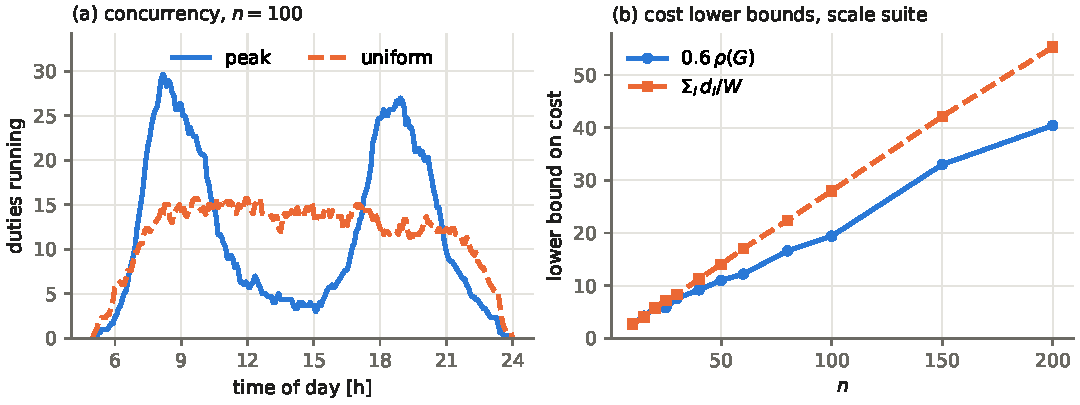
\includegraphics[width=\textwidth]{figures/instances.pdf}
\caption{(a) Number of duties running during the day under the two time
profiles ($n=100$, average of 3 seeds). (b) The two lower bounds on the
optimal cost in the scale group.}
\label{fig:instances}
\end{figure}

\paragraph{Observations.}
\begin{itemize}
  \item \emph{Size.} Density stays near $0.64$ in the scale group, so
    $|\A|$ grows quadratically (from 29 arcs at $n=10$ to about 12\,800 at
    $n=200$). With an employee pool of size $\Theta(n)$, (AF) has
    millions of variables at the top of the range. This is a deliberate
    stress test for the compact models.
  \item \emph{Profile.} The peak profile concentrates the duties in two rush
    hours (Figure~\ref{fig:instances}a): maximum concurrency rises from 10.7
    to 14 at $n=40$ and $\rho(G)$ from 12 to 15.3. Since overlapping duties
    need different employees, peaks drive the number of employees.
  \item \emph{Which bound dominates.} For the default class the two bounds
    are close for small $n$, and the working-time bound dominates from
    $n\approx 25$ (Figure~\ref{fig:instances}b). Short duties reverse this
    ($6.0$ vs.\ $4.7$): the binding factor is then the number of parallel
    duties, not the hours. Long duties make the working-time bound clearly
    dominant ($17.9$ vs.\ $11.2$), and $34\%$ of them can only be covered by
    full-time employees. The duration classes thus move instances between a
    ``covering-type'' and a ``packing-type'' regime.
  \item \emph{Spread limit.} $T$ does not change $G$, but it changes how
    much of $G$ a single employee can use: the effective density goes from
    $0.29$ ($T=600$) to $0.64$ ($T=960$).
  \item \emph{Transfer times.} Their effect on the density is mild ($0.66$
    to $0.61$ from low to high): duties last about two hours, much longer
    than the transfers, so most arcs are decided by the time order alone. To
    control the density directly we therefore rely on \texttt{arc\_drop},
    which lowers it to $0.44$ and $0.26$.
  \item \emph{OR-Library.} These instances are much sparser and the
    working-time bound dominates strongly ($\sum d_i/W\approx 3\times
    0.6\rho$). They extend the size range up to $n=500$ on graphs where only
    (AF) is valid.
\end{itemize}
